\documentclass{article}


\usepackage[preprint]{neurips_2026}   % preprint = clean titled paper; use bare/[main] for submission


\usepackage[utf8]{inputenc}
\usepackage[T1]{fontenc}
\usepackage{hyperref}
\usepackage{url}
\usepackage{booktabs}
\usepackage{amsfonts}
\usepackage{amssymb}
\usepackage{amsmath}
\usepackage{graphicx}
\usepackage{float}
\usepackage{microtype}


\title{Reinforcement Learned Planning: Gradient Plan Optimization\\ Guided by a Learned Reward, Not Latent Geometry}


\author{%
  Anonymous Author(s)\\
  Affiliation\\
  \texttt{email}\\
}


\begin{document}


\maketitle


\section{Introduction}

Planning inside a learned world model (WM) is today dominated by \emph{sampling}:
the Cross-Entropy Method (CEM) and MPPI draw hundreds of action sequences, roll
each through the WM, and iterate the sampling distribution toward the low-cost
survivors. This zeroth-order search is robust---it needs only the \emph{ranking}
of sampled plans to be roughly right---but costs thousands of rollouts per
decision and scales badly with plan dimension and horizon, exactly where the
ranking signal thins out. A learned WM is differentiable, so the natural
alternative is first-order: backpropagate a plan cost through the rollout and
descend it in action space. This is rarely used---but not for the reason usually
given. The failure is \emph{not} that WM gradients are uninformative; it is
\emph{what people take the gradient of}. The standard cost is the WM's
\emph{latent structure}: Euclidean distance between predicted-terminal and goal
embeddings. For self-supervised encoders (DINO, LeJEPA, VICReg) this geometry is
not a metric of \emph{reachability}---nearby embeddings need not be few actions
apart---so its gradient points in directions that do not reduce task cost.
Descent stalls in false basins; CEM survives only because coarse ranking
tolerates a mis-shaped landscape a gradient cannot.

Gradient planning must therefore be made into \emph{its own algorithm}, with two
changes. \textbf{(i)~The objective must be a learned reward}: a goal-conditioned
cost-to-go trained for temporal distance, not the encoder's incidental latent
geometry. \textbf{(ii)~The optimizer must be learned}, not vanilla descent: a
compact update rule, trained by backpropagation through the frozen WM, that takes
the value's gradient as a \emph{feature} and learns how to move the plan. We call
the result \textbf{Reinforcement Learned Planning} (RLP). It plans with
$\sim$16 rollout-equivalents per step (vs.\ $\sim$9{,}000 for CEM),
deterministically, and---across two benchmarks and four world models---beats the
sampling planner most exactly where the WM's native latent cost is weakest.


\section{Method}

\textbf{Setup.} A frozen WM $W$ over latents $z$; a plan is $\mathbf A=(A_1,\dots,A_H)$
of $H$ action blocks. From an encoded history the WM unrolls autoregressively,
differentiable in $\mathbf A$: $\hat z_t = W(\hat z_{t-3:t-1}, a_{t-3:t-1})$,
giving the terminal latent $\hat z_H(\mathbf A)$.

\textbf{Critic --- a learned reward (cost-to-go).} $V_\phi(z,z_g)\!\ge\!0$ is a
goal-conditioned temporal distance (quasimetric head), trained \emph{offline} on
logged latents by $n$-step expectile TD with hindsight goals, $\gamma\!=\!1$,
reached flag $r$, true distance $\delta$:
\begin{equation}
y = r\,\delta + (1{-}r)\big(n_{\mathrm{eff}} + V_{\bar\phi}(z_{t+n},z_g)\big),
\quad
\mathcal L_{\mathrm{TD}}(\phi)=\mathbb E\big[\omega_\tau(u)\,\mathrm{Huber}_\beta(u)\big],\;
u=V_\phi(z_t,z_g)-\mathrm{sg}(y),
\end{equation}
with expectile weight $\omega_\tau(u){=}(1{-}\tau)$ if $u{>}0$ else $\tau$, and
$\bar\phi$ an EMA copy. Low $\tau{\ll}0.5$ makes $V$ optimistic toward the
minimum (shortest-path semantics). This learned reward---not the WM's raw latent
distance---is what the planner descends.

\textbf{Actor --- a learned optimizer over plans.} $f_\theta$ is a weight-tied
update rule applied $K$ times from the zero plan:
\begin{equation}
\mathbf A^{(0)}{=}\mathbf 0,\qquad
\mathbf A^{(k+1)}=\mathrm{clip}\!\big(\mathbf A^{(k)}+f_\theta(\mathbf A^{(k)},\,\widehat{\nabla_{\!\mathbf A}V},\,E,\,k)\big),
\quad E=V(\hat z_H(\mathbf A^{(k)}),z_g),
\end{equation}
where $\widehat{\nabla_{\!\mathbf A}V}$ is the RMS-normalized gradient of the
terminal value through the frozen WM. The goal enters \emph{only} through $V$ and
its gradient---never as raw latent geometry---so the rule is reachability-guided
by construction; no descent prior is hard-coded. $\theta$ is trained purely
pathwise (no RL, no behavior cloning) by backpropagating the terminal value
through the whole $K$-step chain and the frozen rollouts:
$\mathcal L_{\mathrm{actor}}(\theta)=\mathbb E[\,V(\hat z_H(\mathbf A^{(K)}),z_g)+\lambda\,\tfrac1K\sum_k V(\hat z_H(\mathbf A^{(k)}),z_g)\,]$.
Critic and actor train in tandem with strict gradient separation ($\mathcal
L_{\mathrm{actor}}$ never updates $\phi$); at deploy, $K$ refinements from
$\mathbf A^{(0)}{=}\mathbf 0$, execute, replan---no sampling, no restarts.

\begin{figure}[t]
\centering
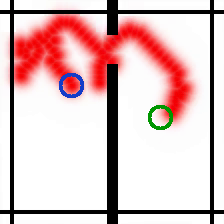
\includegraphics[height=1.45in]{tworoom_traj.png}\hspace{0.5em}
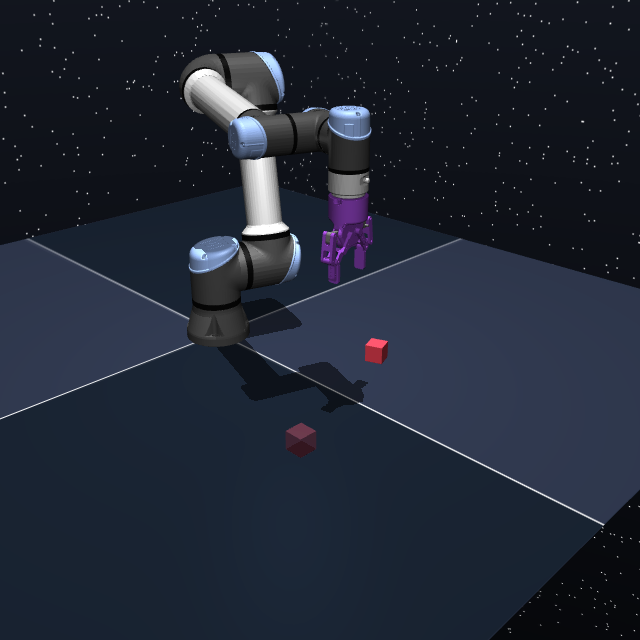
\includegraphics[height=1.45in]{cube_0.png}\hspace{0.5em}
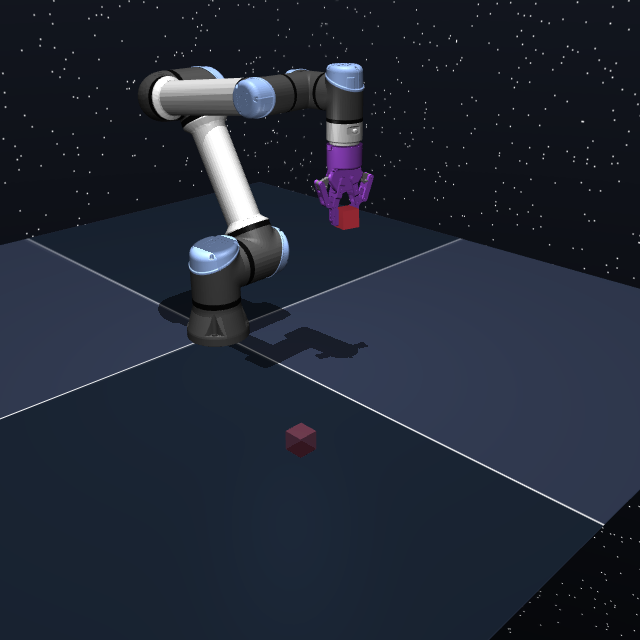
\includegraphics[height=1.45in]{cube_1.png}
\caption{Benchmarks. \emph{Left:} a full RLP trajectory on TwoRoom's hard
setting (h50, cross-wall goal): from the start (blue ring) the agent detours
through the door gap to reach the goal room (goal $=$ green ring); the red
trail is the agent's actual path, composited over the episode. \emph{Middle,
right:} OGBench cube --- the arm must grasp the red block and place it within
4\,cm of the goal pose (translucent cube), shown at the start and mid-transport.
RLP plans in each WM's frozen latent space from pixels/proprio only.}
\label{fig:envs}
\end{figure}


\section{Results}

The baseline is the \emph{no-move} (zero-action) policy---the agent does
nothing---so success reflects only what \emph{planning} contributes. All numbers
are image-based planning, mean over 3 eval-seed task draws $\times$ 50 tasks,
identical draws across planners; RLP uses the \emph{same} learned-optimizer
architecture on every WM, only the frozen WM changes. Tables~\ref{tab:resc}
and~\ref{tab:raw} give the OGBench cube result two ways: floor-rescaled (the
no-move floor is set to $0\%$ and a perfect policy to $100\%$, so each entry is
the fraction of above-floor headroom captured) and raw success with the floor as
a base row. Horizon $=$ goal offset in primitive steps; CEM $=$ the WM's native
latent-distance cost searched by CEM ($\sim$9{,}000 rollouts), RLP $=$ ours
($\sim$16).

\begin{table}[H]
\caption{OGBench cube, floor-rescaled (no-move $=0\%$, perfect $=100\%$):
fraction of above-floor headroom captured. RLP dominates at both horizons, most
on the weaker PLDM world model.}
\label{tab:resc}
\centering\small
\begin{tabular}{l cc c cc}
\toprule
& \multicolumn{2}{c}{LeWM (LeJEPA)} & & \multicolumn{2}{c}{PLDM}\\
\cmidrule(lr){2-3}\cmidrule(lr){5-6}
planner & h25 & h75 & & h25 & h75\\
\midrule
no-move floor & 0 & 0 & & 0 & 0\\
Native CEM (latent) & 55 & 41 & & 35 & 26\\
\textbf{RLP (ours)} & \textbf{81} & \textbf{78} & & \textbf{57} & \textbf{43}\\
\bottomrule
\end{tabular}
\end{table}

\begin{table}[H]
\caption{OGBench cube, raw success (\%), with the no-move floor as a base row
(block within 4\,cm of goal).}
\label{tab:raw}
\centering\small
\begin{tabular}{l cc c cc}
\toprule
& \multicolumn{2}{c}{LeWM (LeJEPA)} & & \multicolumn{2}{c}{PLDM}\\
\cmidrule(lr){2-3}\cmidrule(lr){5-6}
planner & h25 & h75 & & h25 & h75\\
\midrule
no-move floor & 44.7 & 46.0 & & 44.7 & 46.0\\
Native CEM (latent) & 75.3 & 68.0 & & 64.0 & 60.0\\
\textbf{RLP (ours)} & \textbf{89.3} & \textbf{88.0} & & \textbf{76.3} & \textbf{69.3}\\
\bottomrule
\end{tabular}
\end{table}

\begin{table}[H]
\caption{TwoRoom navigation, raw success (\%); std / hard $=$ same-room /
across-the-wall goals. LeWM row is the 3-seed result; PLDM the released
pretrained base.}
\label{tab:tr}
\centering\small
\begin{tabular}{l ccccc}
\toprule
planner & std\,h25 & std\,h50 & hard\,h25 & hard\,h50 & overall\\
\midrule
no-move floor & 10.0 & 1.3 & 1.3 & 0.0 & 3.2\\
Latent+CEM & 84.0 & 58.0 & 82.7 & 68.0 & 73.2\\
\textbf{RLP (LeWM)} & \textbf{100.0} & \textbf{100.0} & \textbf{100.0} & \textbf{100.0} & \textbf{100.0}\\
\textbf{RLP (PLDM)} & 90.7 & 95.3 & 97.3 & 96.7 & 95.0\\
\bottomrule
\end{tabular}
\end{table}

\paragraph{Efficiency (compute vs.\ wall-clock).} RLP reaches a plan with
$\approx$16 WM rollout-equivalents per decision ($K$ refinement steps $\times$ 2
rollouts) versus CEM's $\approx$9{,}000 (300 samples $\times$ 30 iterations): a
$\sim$560$\times$ reduction in world-model compute, deterministically. Measured
wall-clock (same env, same WM, h75) is $\approx$1.1\,s per replan for RLP versus
$\approx$9\,s for CEM---$\sim$8$\times$ faster. The wall-clock gap is far smaller
than the compute gap only because CEM batches its 300 samples in parallel each
iteration while \emph{RLP is not parallelized yet}: its $K$ refinement rollouts
and per-environment plans run serially. Batching them closes most of that gap, so
$\sim$8$\times$ is a floor, not a ceiling.

\paragraph{Findings.} (1)~One learned-optimizer architecture transfers unchanged
across four world models (two objectives $\times$ two benchmarks) and beats the
sampling planner on every horizon. (2)~RLP's advantage is largest exactly where
the WM's latent cost is weakest (PLDM $<$ LeWM), and on LeWM-cube it holds with
horizon as raw latent guidance decays but the learned reward does not. (3)~It
does so at $\sim$560$\times$ less planning compute than CEM. Together: gradient
planning works once it is given a learned reward and a learned optimizer instead
of the encoder's latent geometry and vanilla descent.

\paragraph{Notes.} $0=$ no-move (zero-action) policy. Cube LeWM h25 RLP $=$
89.3 (3-seed mean) on the negative-data (grasp-miss) fine-tuned LeWM with a
negatives-augmented critic; on the authors' stock checkpoint RLP $=$ 88.0. The
h75 column and all CEM baselines use the stock checkpoint. PLDM cube $=$ 2-seed
mean. TwoRoom LeWM $=$ the LeWM-TwoRoom checkpoint, 100 on all 12 cells
$\times$ 3 seeds (the authors' released ``lejepa'' pretrained variant reaches
99.3); PLDM $=$ released pretrained base, single seed. Latent+CEM is on the
LeWM WM.


\end{document}
